%Herramientas elementales para cargar y manipular datos en Python con Pandas. Formatos principales para guardar datos y sus diferencias.

\documentclass[11pt,t,aspectratio=169]{beamer}
\usepackage{borelian}
\usepackage{multirow}


\begin{document}
\classtitle{7}{Manejo de Datos en Python.}


%%%%%%%
\begin{frame}{Contenidos de hoy}
    
    \begin{itemize}%[<+->]
        \item Introducción a Pandas en Python.
        
        \item Estructuras de Datos en Pandas (Series y DataFrames).
        
        \item Como cargar datos en Pandas.

        \item Como acceder a datos en Pandas.
        
        \item Como guardar datos en Pandas.
    
        

    \end{itemize}
    
\end{frame}


%%%%%%%
\begin{frame}{Paquete Pandas en Python}
    Pandas es una librería muy flexible que permite manejar y visualizar datos. 
\vspace{5mm}
    \begin{itemize}
        \item Contiene estructuras y herramientas para manejar datos de manera conveniente.

        \item Tiene metodos para visualizar datos.
    \end{itemize}

\vspace{5mm}
\textbf{Por que Pandas ?}
    \begin{itemize}
        \item Contiene estructuras y herramientas para manejar datos de manera conveniente.
        \item Es mucho mas flexible que otros programas (ej. Excel), por lo que nos permite hacer cosas mas complicadas y útiles para aplicaciones de IA.
        \item Es capaz de manejar grandes datasets con muchos ejemplos.
    \end{itemize}

\end{frame}



\begin{frame}[fragile]{Empezando con Pandas}

Primero importamos el paquete para hacer uso de todas sus funciones.

\begin{minted}{python}
import pandas # importamos el paquete
data = pandas.read_csv("datos.csv") #usamos las funciones del paquete
\end{minted}

Existe una manera mas conveniente de hacer esto. 
\begin{minted}{python}
import pandas as pd # importamos el paquete
data = pd.read_csv("datos.csv") #usamos las funciones del paquete
\end{minted}
\paragraph{Así, evitamos escribir $\code{pandas}$ en cada llamada a una función. También, comúnmente usaremos la librería $\code{numpy}$ en conjunto con pandas.}

\begin{minted}{python}
import numpy as np
\end{minted}


\end{frame}


%%%%%%%%%%%%%%%%%%%%%%%%%%%% DICCIONARIOS %%%%%%%%%%%%%%%%%%%%%%%%%%%%%%%%


\begin{frame}[fragile]
{Antes de Pandas: Diccionarios.}
El diccionario es una estructura de datos que almacena datos en forma \textbf{\emph{llave:valor}}. 

\begin{minted}{python}
>>> country_capitals = {
  "Germany": "Berlin",  # item 1
  "Canada": "Ottawa",   # item 2
  "England": "London",  # item 3
  }

>>> country_capitals["Canada"] # buscamos la capital de Canada
\end{minted}

%\begin{figure}
%    \centering
%    \includegraphics[width=1.5\linewidth]{days/03/image/python_dictionary-example.png}
%    %\caption{Pokemones de primera generación.}
%    \label{fig:placeholder}
%\end{figure}
   
\end{frame}




%%%%%%%%%%%%%%%%%%%%%%%%%%%% PANDAS %%%%%%%%%%%%%%%%%%%%%%%%%%%%%%%%
\begin{frame}{Estructuras de Datos en Pandas.}
    Usando diccionarios podemos crear nuevas estructuras de datos. Por ejemplo, \textbf{Series y DataFrames}.

    \begin{table}[]
        \centering
        \begin{tabular}{c|c|c}
            Dim & Nombre & Descripción \\
            \hline
            1D & \code{pd.Serie} & Arreglo de elementos 1D de un solo tipo \\
            2D & \code{pd.DataFrame} & Arreglo 2D etiquetado mutable con columnas de tipo Serie.
        \end{tabular}
        \caption{Tipos de estructuras de datos en Pandas.}
        \label{tab:placeholder}
    \end{table}

    
\end{frame}



%%%%%%%%%%%%%%%%%%%%%%%%%%%% SERIES %%%%%%%%%%%%%%%%%%%%%%%%%%%%%%%%
\begin{frame}[fragile]{Objetos de tipo Series}
Un objeto de tipo \emph{Series} es un arreglo 1-dimensional que contiene una secuencia de valores del mismo tipo. Este arreglo tiene asociado un arreglo de etiquetas, llamado \emph{index}. 

\begin{figure}[H]
\centering
\includegraphics[width=0.2\linewidth]{days/03/image/series.png}
\caption{Ejemplo de Series.}
\end{figure}

\end{frame}



\begin{frame}[fragile]{Objetos de tipo Series}
Un objeto de tipo \emph{Series} es un arreglo 1-dimensional que contiene una secuencia de valores del mismo tipo. Este arreglo tiene asociado un arreglo de etiquetas, llamado \emph{index}. 

\begin{itemize}
    \item Podemos crear un objeto \emph{Series} usando un diccionario. 
\end{itemize}

\begin{minted}{python}
>>> dicc = {"a":3,"b":2,"c":1} 
>>> obj = pd.Series(dicc)
>>> obj
\end{minted}

Retorna
\begin{minted}{python}
a 3
b 2
c 1
dtype: int64
\end{minted}
\end{frame}

\begin{frame}[fragile]{Objetos de tipo Series}
Un objeto de tipo \emph{Series} es un arreglo 1-dimensional que contiene una secuencia de valores del mismo tipo. Este arreglo tiene asociado un arreglo de etiquetas, llamado \emph{index}. 

\begin{itemize}
    \item Podemos crear un objeto \emph{Series} usando una lista.  
\end{itemize}

\begin{minted}{python}
>>> obj = pd.Series([4, 7, -5, 3])
>>> obj
\end{minted}

Retorna
\begin{minted}{python}
0 4
1 7
2 -5
3 3
dtype: int64
\end{minted}
\end{frame}


%%%%%%%%%%%%%%%%%%%%%%%%%%%%%%

\begin{frame}[fragile]{Objetos de tipo DataFrame}
Un objeto de tipo \emph{DataFrame} representa una tabla rectangular de datos. Esta contiene una colección de columnas, donde cada una puede ser de un tipo diferente.

\begin{figure}[H]
\centering
\includegraphics[width=0.2\linewidth]{days/03/image/dataframes.png}
\caption{Ejemplo de Series.}
\end{figure}
    
\end{frame}



\begin{frame}[fragile]{Objetos de tipo DataFrame}
Un objeto de tipo \emph{DataFrame} representa una tabla rectangular de datos. Esta contiene una colección de columnas, donde cada una puede ser de un tipo diferente.

\begin{itemize}
    \item Podemos crear un objeto \emph{DataFrame} usando un diccionario donde cada \emph{item} representa una columna. 
\end{itemize}

\begin{columns}
    \column{0.5\textwidth}

\begin{minted}{python}
data = {
"Name": ["Alice", "Bob", "Charlie"],
"Age": [25, 30, 35],
"City": ["Berlin", "Ottawa", "Londres"]
}
df = pd.DataFrame(data)
df
\end{minted}   
    
    \column{0.5\textwidth}

\begin{figure}
\centering
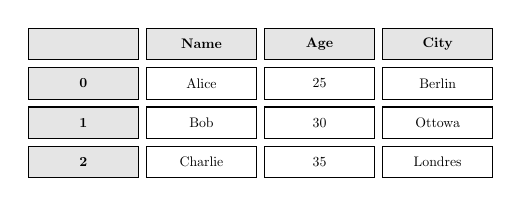
\begin{tikzpicture}[scale=0.5, transform shape,
    cell/.style={
        draw,
        minimum width=2.8cm,
        minimum height=0.8cm,
        align=center
    },
    header/.style={
        cell,
        fill=gray!20,
        font=\bfseries
    }
]

% --- Headers ---
\node[header] (h0) at (0,0) {};
\node[header] (h1) at (3,0) {Name};
\node[header] (h2) at (6,0) {Age};
\node[header] (h3) at (9,0) {City};

% --- Row 0 ---
\node[header] at (0,-1) {0};
\node[cell] at (3,-1) {Alice};
\node[cell] at (6,-1) {25};
\node[cell] at (9,-1) {Berlin};

% --- Row 1 ---
\node[header] at (0,-2) {1};
\node[cell] at (3,-2) {Bob};
\node[cell] at (6,-2) {30};
\node[cell] at (9,-2) {Ottowa};

% --- Row 2 ---
\node[header] at (0,-3) {2};
\node[cell] at (3,-3) {Charlie};
\node[cell] at (6,-3) {35};
\node[cell] at (9,-3) {Londres};

\end{tikzpicture}
%\caption{Representación gráfica de un DataFrame de Pandas}
\end{figure}

\end{columns}
    
\end{frame}


\begin{comment}
\begin{frame}[fragile]{Objetos de tipo DataFrame}
    Un objeto de tipo \emph{DataFrame} representa una tabla rectangular de datos. Esta contiene una colección de columnas, donde cada una puede ser de un tipo diferente.  
    
    \begin{minted}{python}
    In[1]: data = {"state": ["Ohio", "Ohio", "Ohio", "Nevada", "Nevada"],
    "year": [2000, 2001, 2002, 2002, 2003],
    "pop": [1.5, 1.7, 3.6, 2.9, 3.2]}
    In[2]: frame = pd.DataFrame(data)
\end{minted}

\begin{minted}{python}
Out[2]:
state year pop
0 Ohio 2000 1.5
1 Ohio 2001 1.7
2 Ohio 2002 3.6
3 Nevada 2002 2.9
4 Nevada 2003 3.2
\end{minted}    
\end{frame}
\end{comment}


\begin{frame}{DataFrames a partir de datasets}


\paragraph{En los ejemplos anteriores generamos Series y DataFrames usando datos creados de manera manual. Sin embargo, en proyectos reales debemos cargar datos desde datasets o paginas webs. Esto se puede realizar con las siguientes funciones (Tabla \ref{tab:read_data}).}

\begin{table}[h]
\centering
\begin{tabular}{c|p{6cm}|p{5cm}}
\hline
\textbf{Función} & \textbf{Uso} & \textbf{Ejemplo} \\
\hline

\multirow{2}{*}{$\code{read\_csv}$}
& \multirow{2}{6cm}{Cargar datos delimitados por comas desde un archivo local o una URL}
& \multirow{2}{*}{$\code{pd.read\_csv("datos.csv")}$}  \\
&  \\
\hline

\multirow{2}{*}{$\code{read\_excel}$}
& \multirow{2}{6cm}{Cargar datos tabulares desde un archivo Excel}
& \multirow{2}{*}{$\code{pd.read\_excel("datos.xlsx")}$} \\
&  \\
\hline

\multirow{2}{*}{$\code{read\_pickle}$}
& \multirow{2}{6cm}{Cargar datos serializados en formato pickle}
& \multirow{2}{*}{$\code{pd.read\_pickle("datos.pkl")}$} \\
&  \\
\hline

\multirow{2}{*}{$\code{read\_json}$}
& \multirow{2}{6cm}{Cargar datos desde archivos JSON}
& \multirow{2}{*}{$\code{pd.read\_json("datos.json")}$} \\
&  \\
\hline

\end{tabular}
\caption{Funciones de Pandas para carga de datos}
\label{tab:read_data}
\end{table}
\end{frame}


%%%%%%%%%%%%%%%%%%%%%%%%%%%%%%%%%%%%%%% BASICOS DE PANDAS %%%%%%%%%%%%%%%%%%%%%%%%%%%%%%%%%%%%%%%%%%%%%%%%%%%%%%%%%%%%%

\begin{frame}[fragile]{Básicos de Pandas}

Ahora veremos que cosas basicas podemos hacer con un DataFrame. Volveremos a crear un pequeño dataset. 

\begin{minted}{python}
data = {
"Name": ["Alice", "Bob", "Charlie", "Kim"],
"Age": [45, 50, 35, 20],
"City": ["Berlin", "Ottawa", "Londres", "Hong Kong"]
}
df = pd.DataFrame(data)
df
\end{minted}   
    
\begin{figure}
\centering
\input{tikz_figure/df_base.tex}
%\caption{Representación gráfica de un DataFrame de Pandas}
\end{figure}

\end{frame}


%%%%%%%%%%%%%%%%%%%%%%%%%%%%%%%% METODOS DATAFRAME %%%%%%%%%%%%%%%%%%%%%%%%%%%%%%%%%%%%


\begin{frame}[fragile]{Metodo Head}

\begin{itemize}
    \item $\code{df.head()}$ para mirar las primeras filas.
\end{itemize}

\begin{figure}
\centering
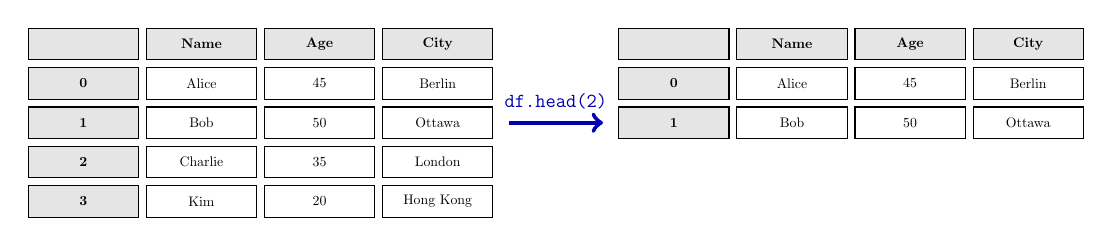
\begin{tikzpicture}[scale=0.5, transform shape,
    cell/.style={
        draw,
        minimum width=2.8cm,
        minimum height=0.8cm,
        align=center
    },
    header/.style={
        cell,
        fill=gray!20,
        font=\bfseries
    }
]

%%%%%%%%%%%%%%%%%%%%%%%%
% DataFrame original
%%%%%%%%%%%%%%%%%%%%%%%%

% --- Headers ---
\node[header] (h0) at (0,0) {};
\node[header] (h1) at (3,0) {Name};
\node[header] (h2) at (6,0) {Age};
\node[header] (h3) at (9,0) {City};

% --- Row 0 ---
\node[header] at (0,-1) {0};
\node[cell] at (3,-1) {Alice};
\node[cell] at (6,-1) {45};
\node[cell] at (9,-1) {Berlin};

% --- Row 1 ---
\node[header] at (0,-2) {1};
\node[cell] at (3,-2) {Bob};
\node[cell] at (6,-2) {50};
\node[cell] at (9,-2) {Ottawa};

% --- Row 2 ---
\node[header] at (0,-3) {2};
\node[cell] at (3,-3) {Charlie};
\node[cell] at (6,-3) {35};
\node[cell] at (9,-3) {London};

% --- Row 3 ---
\node[header] at (0,-4) {3};
\node[cell] at (3,-4) {Kim};
\node[cell] at (6,-4) {20};
\node[cell] at (9,-4) {Hong Kong};

%%%%%%%%%%%%%%%%%%%%%%%%
% Flecha df.head(2)
%%%%%%%%%%%%%%%%%%%%%%%%

\draw[->, ultra thick, blue!70!black]
    (10.8,-2)
    to[out=0,in=180]
    node[midway, above=6pt, font=\ttfamily\Large, text=blue!70!black]
    {df.head(2)}
    (13.2,-2);

%%%%%%%%%%%%%%%%%%%%%%%%
% Resultado df.head(2)
%%%%%%%%%%%%%%%%%%%%%%%%

% --- Headers ---
\node[header] at (15,0) {};
\node[header] at (18,0) {Name};
\node[header] at (21,0) {Age};
\node[header] at (24,0) {City};

% --- Row 0 ---
\node[header] at (15,-1) {0};
\node[cell] at (18,-1) {Alice};
\node[cell] at (21,-1) {45};
\node[cell] at (24,-1) {Berlin};

% --- Row 1 ---
\node[header] at (15,-2) {1};
\node[cell] at (18,-2) {Bob};
\node[cell] at (21,-2) {50};
\node[cell] at (24,-2) {Ottawa};

\end{tikzpicture}

\end{figure}
\end{frame}


\begin{frame}[fragile]{Metodo tail}
\begin{itemize}
    \item $\code{df.tail()}$ para mirar las ultimas filas.
\end{itemize}
\begin{figure}
\centering
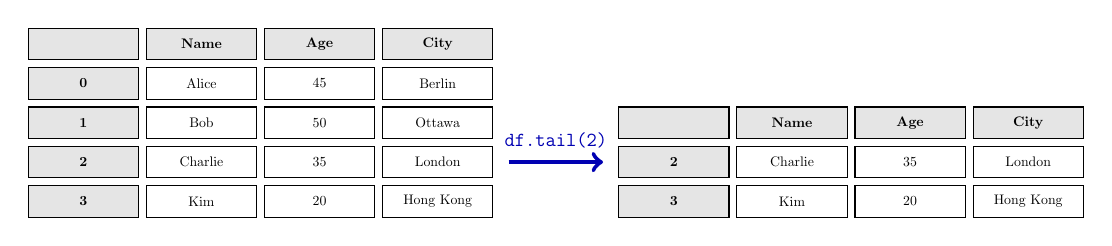
\begin{tikzpicture}[
    scale=0.5, 
    transform shape,
    cell/.style={
        draw,
        minimum width=2.8cm,
        minimum height=0.8cm,
        align=center
    },
    header/.style={
        cell,
        fill=gray!20,
        font=\bfseries
    }
]
    % --- Headers ---
    \node[header] (h0) at (0,0) {};
    \node[header] (h1) at (3,0) {Name};
    \node[header] (h2) at (6,0) {Age};
    \node[header] (h3) at (9,0) {City};

    % --- Row 0 ---
    \node[header] at (0,-1) {0};
    \node[cell] at (3,-1) {Alice};
    \node[cell] at (6,-1) {45};
    \node[cell] at (9,-1) {Berlin};

    % --- Row 1 ---
    \node[header] at (0,-2) {1};
    \node[cell] at (3,-2) {Bob};
    \node[cell] at (6,-2) {50};
    \node[cell] at (9,-2) {Ottawa};

    % --- Row 2 ---
    \node[header] at (0,-3) {2};
    \node[cell] at (3,-3) {Charlie};
    \node[cell] at (6,-3) {35};
    \node[cell] at (9,-3) {London};

    % --- Row 3 ---
    \node[header] at (0,-4) {3};
    \node[cell] at (3,-4) {Kim};
    \node[cell] at (6,-4) {20};
    \node[cell] at (9,-4) {Hong Kong};

    \draw[->, ultra thick, blue!70!black]
        (10.8,-3)
        to[out=0,in=180]
        node[midway, above=6pt, font=\ttfamily\Large] {df.tail(2)}
        (13.2,-3);

    % Result of df.tail(2)
    \node[header] at (15,-2) {};
    \node[header] at (18,-2) {Name};
    \node[header] at (21,-2) {Age};
    \node[header] at (24,-2) {City};

    % --- Row 2 ---
    \node[header] at (15,-3) {2};
    \node[cell] at (18,-3) {Charlie};
    \node[cell] at (21,-3) {35};
    \node[cell] at (24,-3) {London};

    % --- Row 3 ---
    \node[header] at (15,-4) {3};
    \node[cell] at (18,-4) {Kim};
    \node[cell] at (21,-4) {20};
    \node[cell] at (24,-4) {Hong Kong};
\end{tikzpicture}

\end{figure}
\end{frame}

\begin{frame}[fragile]{Atributo shape}
\begin{itemize}
    \item $\code{df.shape}$ devuelve la forma del DataFrame (filas,columnas).
\end{itemize}
\begin{figure}
\centering
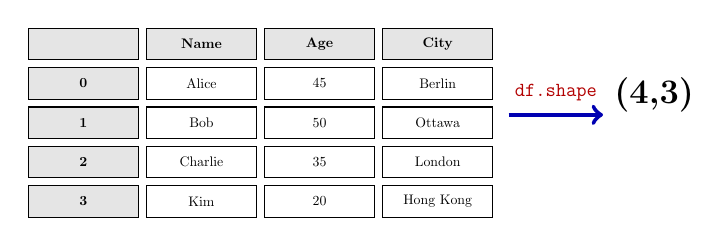
\begin{tikzpicture}[scale=0.5, transform shape,
    cell/.style={
        draw,
        minimum width=2.8cm,
        minimum height=0.8cm,
        align=center
    },
    header/.style={
        cell,
        fill=gray!20,
        font=\bfseries
    }
]

%%%%%%%%%%%%%%%%%%%%%%%%
% DataFrame original
%%%%%%%%%%%%%%%%%%%%%%%%

% --- Headers ---
\node[header] at (0,0) {};
\node[header] at (3,0) {Name};
\node[header] at (6,0) {Age};
\node[header] at (9,0) {City};

% --- Row 0 ---
\node[header] at (0,-1) {0};
\node[cell] at (3,-1) {Alice};
\node[cell] at (6,-1) {45};
\node[cell] at (9,-1) {Berlin};

% --- Row 1 ---
\node[header] at (0,-2) {1};
\node[cell] at (3,-2) {Bob};
\node[cell] at (6,-2) {50};
\node[cell] at (9,-2) {Ottawa};

% --- Row 2 ---
\node[header] at (0,-3) {2};
\node[cell] at (3,-3) {Charlie};
\node[cell] at (6,-3) {35};
\node[cell] at (9,-3) {London};

% --- Row 3 ---
\node[header] at (0,-4) {3};
\node[cell] at (3,-4) {Kim};
\node[cell] at (6,-4) {20};
\node[cell] at (9,-4) {Hong Kong};

%%%%%%%%%%%%%%%%%%%%%%%%
% Flecha df.iloc[0]
%%%%%%%%%%%%%%%%%%%%%%%%

\draw[->, ultra thick, blue!70!black]
    (10.8,-1.8)
    to[out=0,in=180]
    node[midway, above=6pt,
          font=\ttfamily\Large,
          text=red!70!black]
    {df.shape}
    (13.2,-1.8);

%%%%%%%%%%%%%%%%%%%%%%%%
% Resultado df.iloc[0] como Series
%%%%%%%%%%%%%%%%%%%%%%%%

% Título
\node[font=\bfseries\Huge] at (14.5,-1.3) { (4,3) };

%\node[font=\ttfamily\small] at (19.5,-4.2) {Name: 0};

\end{tikzpicture}

\end{figure}
\end{frame}


\begin{frame}[fragile]{Funcion len}
\begin{itemize}
    \item $\code{len(df)}$ devuelve el largo del DataFrame medido en numero de filas.
\end{itemize}
\begin{figure}
\centering
\input{len}
\end{figure}
\end{frame}

\begin{frame}[fragile]{Atributo columns}
\begin{itemize}
    \item $\code{df.columns}$ devuelve los nombres de todas las columnas del DataFrame.
\end{itemize}
\begin{figure}
\centering
\input{columns}
\end{figure}
\end{frame}


\begin{frame}[fragile]{Metodo iloc}

\begin{itemize}
    \item $\code{df.iloc(k)}$ devuelve una Serie generada con la fila en la posición $k$.
\end{itemize}

\begin{figure}
\centering
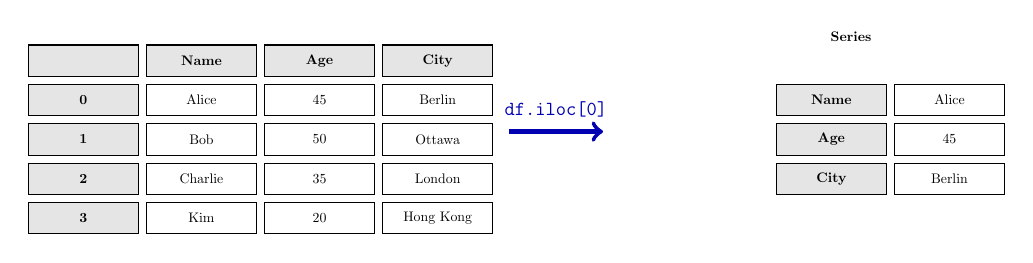
\begin{tikzpicture}[scale=0.5, transform shape,
    cell/.style={
        draw,
        minimum width=2.8cm,
        minimum height=0.8cm,
        align=center
    },
    header/.style={
        cell,
        fill=gray!20,
        font=\bfseries
    }
]

%%%%%%%%%%%%%%%%%%%%%%%%
% DataFrame original
%%%%%%%%%%%%%%%%%%%%%%%%

% --- Headers ---
\node[header] at (0,0) {};
\node[header] at (3,0) {Name};
\node[header] at (6,0) {Age};
\node[header] at (9,0) {City};

% --- Row 0 ---
\node[header] at (0,-1) {0};
\node[cell] at (3,-1) {Alice};
\node[cell] at (6,-1) {45};
\node[cell] at (9,-1) {Berlin};

% --- Row 1 ---
\node[header] at (0,-2) {1};
\node[cell] at (3,-2) {Bob};
\node[cell] at (6,-2) {50};
\node[cell] at (9,-2) {Ottawa};

% --- Row 2 ---
\node[header] at (0,-3) {2};
\node[cell] at (3,-3) {Charlie};
\node[cell] at (6,-3) {35};
\node[cell] at (9,-3) {London};

% --- Row 3 ---
\node[header] at (0,-4) {3};
\node[cell] at (3,-4) {Kim};
\node[cell] at (6,-4) {20};
\node[cell] at (9,-4) {Hong Kong};

%%%%%%%%%%%%%%%%%%%%%%%%
% Flecha df.iloc[0]
%%%%%%%%%%%%%%%%%%%%%%%%

\draw[->, ultra thick, blue!70!black]
    (10.8,-1.8)
    to[out=0,in=180]
    node[midway, above=6pt,
          font=\ttfamily\Large,
          text=blue!70!black]
    {df.iloc[0]}
    (13.2,-1.8);

%%%%%%%%%%%%%%%%%%%%%%%%
% Resultado df.iloc[0] como Series
%%%%%%%%%%%%%%%%%%%%%%%%

% Título
\node[font=\bfseries] at (19.5,0.6) {Series};

% Celdas de la serie (índice, valor)
\node[header] at (19,-1) {Name};
\node[cell] at (22,-1) {Alice};

\node[header] at (19,-2) {Age};
\node[cell] at (22,-2) {45};

\node[header] at (19,-3) {City};
\node[cell] at (22,-3) {Berlin};

% Nombre del índice
%\node[font=\ttfamily\small] at (19.5,-4.2) {Name: 0};

\end{tikzpicture}

\end{figure}
\end{frame}


\begin{frame}[fragile]{Metodo loc}

\begin{itemize}
    \item $\code{df.loc(k)}$ devuelve una Serie generada con la fila indexada por el valor $k$.
\end{itemize}

\begin{figure}
\centering
\input{loc}
\end{figure}
\end{frame}



    %\item $\code{df.shape}$ para obtener las dimensiones de la tabla.
    %\item $\code{len(df)}$ para obtener el numero de filas en la tabla.
    %\item $\code{df.columns}$ para obtener los nombres de las columnas en la tabla.
    %\item $\code{df.iloc[ k ]}$ para obtener la fila ubicada en la posición $k$.
    %\item $\code{df.loc[index]}$ para obtener la fila asignada al indice $index$.


%%%%%%%%%%%%%%%%%%%%%%%%%%%%%%%%%%%%%%%%%%%



\begin{frame}{Como guardar datos con Pandas ?}

Lo ultimo que vamos a ver es como guardar un objeto de tipo DataFrame, podemos guardar este usando las siguientes funciones (Tabla \ref{tab:save_data}).

\begin{table}[h]
\centering
\begin{tabular}{c|p{6cm}|p{5cm}}
\hline
\textbf{Función} & \textbf{Uso} & \textbf{Ejemplo} \\
\hline

\multirow{2}{*}{$\code{to\_csv}$}
& \multirow{2}{6cm}{Guardar un DataFrame en un archivo delimitado por comas (CSV)}
& \multirow{2}{*}{$\code{df.to\_csv("datos.csv")}$} \\
&  \\
\hline

\multirow{2}{*}{$\code{to\_excel}$}
& \multirow{2}{6cm}{Guardar un DataFrame en un archivo Excel}
& \multirow{2}{*}{$\code{df.to\_excel("datos.xlsx")}$} \\
&  \\
\hline

\multirow{2}{*}{$\code{to\_pickle}$}
& \multirow{2}{6cm}{Serializar y guardar un DataFrame en formato pickle}
& \multirow{2}{*}{$\code{df.to\_pickle("datos.pkl")}$} \\
&  \\
\hline

\multirow{2}{*}{$\code{to\_json}$}
& \multirow{2}{6cm}{Guardar un DataFrame en un archivo JSON}
& \multirow{2}{*}{$\code{df.to\_json("datos.json")}$} \\
&  \\
\hline

\end{tabular}
\caption{Funciones de Pandas para guardar datos}
\label{tab:save_data}
\end{table}

\end{frame}


\begin{frame}{Resumen de DataFrames en Pandas.}

\begin{itemize}
    \item $\code{df.read_csv()}$ para cargar un dataset desde un archivo csv o URL.
    \item $\code{df.head()}$ para mirar las primeras filas.
    \item $\code{df.tail()}$ para mirar las ultimas filas.
    \item $\code{df.shape}$ para obtener las dimensiones de la tabla.
    \item $\code{len(df)}$ para obtener el numero de filas en la tabla.
    \item $\code{df.columns}$ para obtener los nombres de las columnas en la tabla.
    \item $\code{df.iloc[ k ]}$ para obtener la fila ubicada en la posición $k$.
    \item $\code{df.loc[index]}$ para obtener la fila asignada al indice $index$.
    \item $\code{df.to_csv()}$ para guardar el DataFrame en un archivo csv.
\end{itemize}

\textbf{Pandas tiene mas funciones! (veremos esto mañana...)}.
    
\end{frame}


\begin{frame}{Resumen de la clase.}

\begin{itemize}
    \item Diccionarios de Python.
    \item pd.Series de Python.
    \item pd.DataFrames de Python.
    \item Funciones asociadas a la clase pd.DataFrame.
\end{itemize}

\end{frame}

\begin{frame}{Vamos a ver un ejemplo practico en Python Collab}
    Exploremos un dataset: \url{https://colab.research.google.com/drive/1X7xoTisfFrGZFfrQ9ROckTaYzv8Xw8TB?usp=sharing}.

\begin{figure}
    \centering
    \includegraphics[width=0.5\linewidth]{days/03/image/pokemon.png}
    \caption{Pokemones de primera generación.}
    \label{fig:placeholder}
\end{figure}
    
\end{frame}


\begin{frame}{Referencias:}
    \begin{itemize}
        \item Wes McKinney. (2022). Python for Data Analysis. Third Edition.
    \end{itemize}
\end{frame}


\end{document}